\documentclass[pdf,12pt,report,strict]{SANDreport}

\usepackage{amsmath}
\usepackage{amsfonts}
\usepackage{amssymb}
\usepackage{graphicx}
\usepackage{float}
\usepackage{makeidx}
\usepackage{cite}
\usepackage{subfigure}
\usepackage{ifthen}
\usepackage{xspace}
\usepackage{hyperref}

%-----------------------------------------------------------------------------
% My commands
%
\newcommand*{\lcite}[1]{~\cite{#1}}
\newcommand*{\scite}[1]{~\cite{#1}}
\newcommand{\titan}{Titan\index{Titan}\xspace}
\newcommand{\threatview}{ThreatView\texttrademark\index{ThreatView@ThreatView\texttrademark}\xspace}

\newcommand*{\keyterm}[1]{\textbf{#1}}
\newcommand*{\keytermidx}[1]{\keyterm{#1}\index{#1}}

%-----------------------------------------------------------------------------
% My options
%

% Put figures inline with text when possible.
\floatplacement{figure}{htb}

% Avoid putting figures on their own page.
\renewcommand{\textfraction}{0.05}
\renewcommand{\topfraction}{0.95}

% Make sure this is big enough so that only big figures end up on their own
% page but small enough so that if a figure does have to be on its own
% page, it won't push everything to the bottom because it's not big enough
% to have its own page.
\renewcommand{\floatpagefraction}{.75}

\newcommand{\sticky}[1]{\textsc{[#1]}}

\makeindex

% ---------------------------------------------------------------------------- %
% Set the title, author, and date
%
\title{Massive Graph Visualization}
\author{Dr. Kenneth D. Moreland, SMTS\\
Scalable Analytics \& Visualization\\
P.O. Box 5800\\
Albuquerque, NM 87185-1323\\
\\
Brian N. Wylie, PMTS\\
Scalable Analytics \& Visualization\\
P.O. Box 5800\\
Albuquerque, NM 87185-1323}
\date{}					% Leave this here but empty


% ---------------------------------------------------------------------------- %
% These are mandatory
%
\SANDnum{SAND 2007-XXXX}			% e.g. \SANDnum{SAND2006-0420}
\SANDprintDate{}
\SANDauthor{Kenneth~Moreland and Brian~Wylie}	% One line, separated by commas


% ---------------------------------------------------------------------------- %
% These are optional
%
%\SANDrePrintDate{}	% May be repeated for successive printings
%\SANDsupersed{}{}	% {Old SAND number}{Old date}


% ---------------------------------------------------------------------------- %
% Build your markings. See example files and SAND Report Guide
%
% \SANDreleaseType{}
% \SANDmarkTopBottomCoverBackTitle{}
% \SANDmarkBottomCover{}
% \SANDmarkTopBottomCoverTitle{}
% \SANDmarkTop{}
% \SANDmarkBottom{}
% \SANDmarkTopBottom{}
% \SANDmarkCover{}
% \SANDmarkCoverTitle{}


% ---------------------------------------------------------------------------- %
% Start the document
%
\begin{document}
\maketitle

% ------------------------------------------------------------------------ %
% An Abstract is required for SAND reports
% 
\begin{abstract}
  Graphs are a vital way of organizing data with complex correlations. A
  good visualization of a graph can fundamentally change human
  understanding of the data. Consequently, there is a rich body of work on
  graph visualization.  Although there are many techniques that are
  effective on small to medium sized graphs (tens of thousands of nodes),
  there is a void in the research for visualizing massive graphs containing
  millions of nodes. Sandia is one of the few entities in the world that
  has the means and motivation to handle data on such a massive scale. For
  example, homeland security generates graphs from prolific media sources
  such as television, telephone, and the Internet.  The purpose of this
  project is to provide the groundwork for visualizing such massive graphs.
  The research provides for two major feature gaps: a parallel, interactive
  visualization framework and scalable algorithms to make the framework
  usable to a practical application.  Both the frameworks and algorithms
  are designed to run on distributed parallel computers, which are already
  available at Sandia.  Future work will integrate these features into the
  \threatview application.
\end{abstract}


% ------------------------------------------------------------------------ %
% An Acknowledgment section is optional but important
% 
\clearpage
\chapter*{Acknowledgment}

The Massive Graph Visualization LDRD team would like to acknowledge the
significant support provided by Nabeel Rahal, our LDRD program manager.
Without Nabeel's fanatical support, our work may never have left the
ground.  We would like to acknowledge those who provided both direct
and indirect technical development: Timothy Shead and Jeffrey Baumes.  We
also acknowledge Bruce Hendrickson, Jonathan Berry, and Patricia Crossno
for their technical guidance.


% ------------------------------------------------------------------------ %
% The table of contents and list of figures and tables
% 
\cleardoublepage		% TOC needs to start on an odd page
\tableofcontents
\listoffigures
%\listoftables


%% % ---------------------------------------------------------------------- %
%% % An optional preface or Foreword
%% \clearpage
%% \chapter*{Preface}
%% \addcontentsline{toc}{chapter}{Preface}


% ---------------------------------------------------------------------- %
% An optional executive summary
\cleardoublepage		% Executive Summary to start on odd page
\chapter*{Executive Summary}
\addcontentsline{toc}{chapter}{Executive Summary}

The purpose of the project is to develop techniques that enable
understanding of large databases of connected data.  Such databases
naturally form mathematical structures called graphs.  Graphs are a vital
way of organizing data with complex correlations.  A good visualization of
a graph can fundamentally change human understanding of the data.
Consequently, there is a rich body of work on graph visualization.

Although there are many techniques that are effective on small to medium
sized graphs (tens of thousands of nodes), there is a void in the research
for visualizing massive graphs containing millions of nodes.  Sandia is one
of the few entities in the world that has the means and motivation to
handle data on such a massive scale.  For example, homeland security
generates graphs from prolific media sources such as television, telephone,
and the Internet.

\begin{figure}
  \centering
  (Data~Collection) $\rightarrow$ (Entity~Extraction)
  (Event~Similarity~Calculation) (Semantic~Analysis) $\rightarrow$
  (Database)
  \\
  See the original proposal slides for the basic idea.
  \caption{Graph extraction from raw data.}
  \label{fig:GraphExtraction}
\end{figure}

As demonstrated in Figure~\ref{fig:GraphExtraction}, the graphs with which
homeland security must work originate with raw data collected from a
variety of sources.  Data sources of the modern world are far too prolific
to sift through ``by hand.''  Instead, the data is first conditioned by any
number of automated processes such as entity extraction, event similarity
calculation, and semantic analysis.  The result is a set of entities that
are stored in a database in such a way that relationships are easily
retrieved or extracted.  These relations between entities in the database
fundamentally form a graph.  The large size of the input data collection
yields a similarly large graph database; millions of nodes are not
uncommon.

The goal of this project is to facilitate the visualization of such massive
graphs.  We have identified to major fronts of basic research that are
required for practical visual applications: a parallel, interactive
visualization framework and scalable algorithms to make the framework
usable to a practical application.  On both fronts we work with the
constraint that the algorithms must perform well on a distributed memory
parallel machine because of their proven scalability and accessibility
from within Sandia.

\section{Framework}

To build a framework on which to visualize massive graphs, we start with an
already well developed code base.  The field from which we draw from is
\keyterm{scientific visualization}\index{scientific~visualization}.  Scientific
visualization concerns the visualization of meshes, simulation results, and
real-world sensor readings, all of which have a definition in physical
space.  As a world leader in supercomputing for physical simulation, Sandia
has also fostered excellence in scalable parallel scientific visualization.

\index{Visualization Toolkit|see{VTK}}

The framework that Sandia uses to perform scientific visualization is
embedded in \keytermidx{VTK}, the Visualization Toolkit.  VTK provides a
component architecture for visualization components that also provides for
data-centric parallel processing.  Built on top of VTK is
\keytermidx{ParaView}, which provides both a client/server architecture for
parallel interactive visualizations and an end user application for
performing parallel visualizations.

Graph visualization falls under the classification of \keyterm{information
visualization}\index{information~visualization}, which deals with abstract
data types that have no necessary connection to physical space.  ParaView,
designed as a scientific visualization tool, is not equipped to handle this
type of visualization.  However, the distinction between scientific
visualization and information visualization is in many ways artificial.
Many problems in one domain are mirrored in the other.

To leverage many of the features of VTK, including scalable parallel
processing, we started the \keyterm{\titan} project.
The \titan project organizes the work of several funding sources (this LDRD
included) to complement VTK with information visualization capabilities.

\index{edge~partitioning}

The role of this project in \titan is the creation of scalable graph
components.  To accommodate parallel graph structures in a variety of
settings, we built data sets that support edge partitioning, as defined by
Yoo et al.\scite{Yoo05}.  These partitioning structures allow you to divide
the graph data amongst distributed processes and identify where neighboring
vertices are located, the bare minimum for supporting parallel graphs, In
addition, edge partitioning also limits the amount of communication needed
to get neighborhood information and to trace connections within graphs.
This feature can drastically reduce the communication overhead in
algorithms.

The ability to store large graphs in parallel is pointless unless one can
load in data, so our project addressed this as well.  Once data is
processed it is most appropriate to store the entity information in a
database.  Databases are a very well developed technology that provide for
the storage, retrieval and search of large amounts of data.  Although an
active area of research, databases are currently not designed specifically
for graph storage and retrieval.  Most databases store tables of relational
data (although some object-oriented databases exist), and retrievals from
the database are assumed to be tables that are streamed to a single client.

To read in large graphs from databases, we addressed two important issues.
First, we read data from the database in a parallel distributed manner.  We
do this by first instructing the database to save a query in an internal
structure, and then we stream partitions of the table in each process.
Second, we convert the tables into graphs by identifying vertices and
pulling in edges as necessary.

\section{Algorithms}

\index{graph~layout!force~directed|see{force-directed~layout}}

With the framework in place to handle large, parallel graphs, we addressed
the basic algorithms necessary for visualization.  One critical class of
such algorithms are the layout algorithms that impose spatial coordinates
on the graph elements such that their placement suggests the relationships
of the entities.  The most common layout algorithms are
\keyterm{force directed}\index{force-directed~layout}, which places
vertices by minimizing the energy caused by attractive and repulsive forces
defined by the graph structure.  The time to solve this problem completely
grows quadratically with respect to the number of graph nodes.  Good
approximations with better running times exist~\lcite{Hachul04}, but they
are difficult to parallelize efficiently and still have a greater than
linear running time.

\index{graph~layout!fast|see{fast layout}}

We investigated alternative layout algorithms that have a running time that
grows linearly with respect to the number of vertices and edges in the
graph and that can easily be run in parallel.  The first such algorithm,
called simply \keyterm{fast layout}\index{fast~layout}, is a relatively
simple extension to the traditional force directed algorithm.  This
algorithm follows the same basic flow except that the force field is
computed on a finite mesh.  This sampled field can be computed in linear
time with respect to the vertices and can be combined in parallel with a
simple reduce command.

\index{graph~layout!G-Space|see{G-Space}}

The second layout algorithm we designed is the
\keytermidx{G-Space} layout algorithm.  This algorithm differs
significantly from the traditional force-directed layout algorithm.  The
G-Space algorithm first picks two vertices in the graph and performs a
breadth-first search on each to determine the geodesic distance of each
vertex to these two.  These two values form coordinates in a 2D geodesic
space.  The G-Space layout is then based on the plot of the vertices in
geodesic space.

Other algorithms deal with rendering and viewing graphs.  The problem with
viewing large graphs, even those with a good layout, is that the image
quickly becomes saturated.  It can be the case that there are more elements
being rendered than pixels on the screen.  To address this problem, we can
render the elements with the assumption that each is smaller than a screen
pixel.  The fragments then accumulate to show collections of objects.
Although done in the past, we found that the technique, although effective
for vertices, was not subtable for edges.  In response to this, we designed
an algorithm that accumulates edges based on their position and orientation
to get a better idea of when edges bundle together.

Another way to view a large graph is to use a landscape representative of
the density of vertices.  We first derive a sampled field based on the
density of vertices, and then perform a carpet plot of that field.  This
process must be very fast, as it is expected to be updated as we interact
with (pan and zoom) the graph.  We perform this operation using a special
fast splatting algorithm in combination with parallel compositing
techniques.

Once a landscape view is available, it is important to be able to identify
where vertices are.  Given little \emph{a-priori} knowledge, the most
useful information you can give is to identify major clusters.  You can do
that by identifying the peaks in the vertex density field and then placing
an identifying label of a representative vertex there.  Again, the
algorithm we created has to work very fast to maintain interactivity.


%% % ---------------------------------------------------------------------- %
%% % An optional glossary. We don't want it to be numbered
%% \clearpage
%% \chapter*{Nomenclature}
%% \addcontentsline{toc}{chapter}{Nomenclature}
%% \begin{description}
%% \item[Term 1]
%%   Description
%% \item[Term 2]
%%   Description
%% \item[Term 3]
%%   Description
%% \end{description}


% ---------------------------------------------------------------------- %
% This is where the body of the report begins; usually with an Introduction
% 
\SANDmain		% Start the main part of the report

\chapter{Introduction}
\label{chap:Introduction}

The focus of this LDRD was to research the foundations for interactively
analyzing massive graphs.  This problem domain is of particular importance
to homeland security where data accumulated from a variety of independent
sources can quickly form these enormous graphs.  Interactively visualizing
these graphs is vital for detecting threats.

\begin{figure}
  \centering
  In a loop \\
  (Hypothesize) $\rightarrow$ (Query) $\rightarrow$ (Investigate)
  $\rightarrow$ (Conjecture) $\rightarrow$ (Hypothesize)
  \\
  Maybe no conjecture part.
  \caption{Threat Investigation Cycle.}
  \label{fig:ThreatInvestigationCycle}
\end{figure}

Figure~\ref{fig:ThreatInvestigationCycle} shows the cyclical investigation
of threats (a simplification of the \keyterm{analytical reasoning
process}\index{analytical~reasoning~process}\cite{Thomas05}).  An annalist
makes a hypothesis and based on this hypothesis queries the data for
relevant information.  The annalist then investigates and explores this
data.  Based on this investigation, conjectures are drawn and the
hypothesis is modified in accordance to the new information.  The cycle is
repeated with more queries to draw more data about the new information.

Clearly this investigative process relies heavily on the ability to not
only manage this data but to also sift through it quickly.  Several
products have been created to this end\lcite{Hetzler98,Thomas99,Boyack01},
but to date they all are serial applications.  They can handle data of only
a limited scale and are not equipped to deal with graphs on the order of
millions of vertices.  Making the leap to a parallel framework for massive
amounts of data requires the foundational research this LDRD project
provides.

To build scalable graph visualization applications, we first need a
framework on which to build them.  This framework must have the ability to
read, store, and process graphs.  Furthermore, this framework needs to work
well on distributed-memory parallel computers, which are the most easily
scaled and  are already available from within Sandia.  The parallel graph
framework is discussed in
Chapter~\ref{chap:ParallelGraphVisualizationFramework}.

A parallel framework is usable only if we have parallel algorithms to run
on it.  This LDRD project developed some basic parallel graph algorithms
that are fundamental to the visualization of these large graphs.  The
algorithms are discussed in
Chapter~\ref{chap:MassiveGraphVisualizationAlgorithms}.

\section{Related Projects}
\label{sec:RelatedProjects}

This LDRD project is not the only work at Sandia focused on parallel graph
algorithms and large graph visualization.  There are several other projects
in this domain.  Yet each project contributes to a different part of the
solution, and the collective effort is meant to be collaborative rather
than competitive.

\subsection{\titan}
\label{sec:RelatedProjects:Titan}

%\index{Titan@\titan|(}

The \titan project is a coordination of several other projects, this LDRD
included, to merge \index{scientific~visualization}scientific visualization
and \index{information~visualization}information visualization into the
same toolkit: \index{VTK}VTK.  The purpose of \titan is to leverage the
enormous body of work in scientific visualization and jumpstart Sandia's
presence in the information visualization domain.  VTK is mature
open-source tool with a large user base that can contribute back to our
information visualization tools.

This LDRD project provides the necessary tools to make \titan scale to
large, parallel, distributed-memory computers.

%\index{Titan@\titan|)}

\subsection{\threatview}
\label{sec:RelatedProjects:ThreatView}

%\index{ThreatView@\threatview|(}

\index{NGIC|see{National Ground Intelligence Center}}

\threatview is an end user information visualization tool paid for by the
\index{PATTON}PATTON program under the
\index{National~Ground~Intelligence~Center}National Ground Intelligence
Center (NGIC).  \threatview leverages and contributes to \titan for a
modular and extensible architecture.

\threatview also leverages the \index{ParaView}ParaView server libraries
for the ability to interactively run parallel algorithms in client-server
mode.  However, the funding does not include the parallel framework and
algorithms also required for parallel processing.  Instead, \threatview
expects to leverage contributions from other projects (i.e. this LDRD).

%\index{ThreatView@\threatview|)}

\subsection{Multi-Threaded Graph Library}
\label{sec:RelatedProjects:MTGL}

\index{Multi-Threaded~Graph~Library|(}
\index{MTGL|see{Multi-Threaded Graph Library}}

The Multi-Threaded Graph Library (MTGL) is a compendium of parallel graph
algorithms.  The algorithm design is focused on a special class of computer
architecture called massive multithreading.  This architecture has special
hardware to enable each processor to efficiently handle many threads
running memory-access intensive algorithms.  For algorithms that require
repetitive memory requests, which many graph algorithms do, this type of
architecture can be more effective than much larger distributed memory
machines\lcite{Berry07}.

When massive multithreading architectures are available, MTGL can give a
significant performance boost.  Thus, MTGL is being integrated into \titan.
However, massive multithreading computers are rare and expensive.  This
LDRD designed algorithms for the more common distributed-memory machines.
We worked with the knowledge that the architecture has limitations and that
we have to perform with the constraints that we are given.

\index{Multi-Threaded~Graph~Library|)}

\subsection{Parallel Boost Graph Library}
\label{sec:RelatedProjects:PBGL}

\index{Parallel~Boost~Graph~Library|(}
\index{PBGL|see{Parallel Boost Graph Library}}

The Parallel Boost Graph Library (PBGL), developed at Indiana University,
is an extension of the popular Boost Graph Library (BGL) to form parallel
processing of graphs, possibly on distributed-memory
computers\lcite{Gregor05}.

BGL is integrated into \titan and PBGL will soon follow.  However, PBGL, a
library strictly concerned with graph algorithms, is missing the framework
and many algorithms required for interactive parallel visualization.  This
LDRD has not duplicated the work of PBGL, but rather fills gaps needed to
interactively visualize massive graphs.

\index{Parallel~Boost~Graph~Library|)}

\subsection{VxOrd}
\label{sec:RelatedProjects:VxOrd}

\index{VxOrd|(}

VxOrd is a graph layout algorithm that has been developed and tweaked over
many years at Sandia.  Most recently, the VxOrd algorithm has been used in
conjunction with graph coarsening techniques to generate structure from
very large real-world graphs.

The technique is an iterative serial process that takes many hours to
complete on large graphs.  The results can generate stunning visualizations
such as those demonstrating the structure of
science\lcite{Boyack04,Boyack05}.  However, the resulting visualization is
also static.  The layout algorithms designed for this LDRD project lie on
the opposite end of the spectrum.  They are designed to run as fast as
possible even if they do not give the most optimal result.  Such algorithms
are vital for true interactivity.  Users can apply progressively slower
algorithms to further refine the layout as necessary.

\index{VxOrd|)}


\chapter{Parallel Graph Visualization Framework}
\label{chap:ParallelGraphVisualizationFramework}

As part of \titan, this project leverages VTK\index{VTK} for its parallel
graph visualization framework.  The VTK framework, which has supported
parallel scientific visualization for years, is most efficient when running
in \keyterm{data parallelism}\index{data~parallelism} mode.  In this mode, the
data is partitioned and divided amongst all of the processes.

To support data parallelism, our framework must include two things.  We
need data structures that can hold a distributed graph and provide
mechanisms for retrieving connectivity information between processes.  We
also need the ability to load data into the framework.  This means reading
the data from files or querying from databases.  To be scalable, the data
input cannot bottleneck on any one process trying to read the data.

\section{Data Structures}
\label{sec:ParallelGraphVisualizationFramework:DataStructures}

The \titan data structure for holding graphs uses an \keyterm{adjacency
list}\index{adjacency~list} for its representation.  In this
representation, edges are defined with a variable-sized array on each
vertex that points to the vertices to which it connects.  For graphs with
average vertex degree much lower than the total number of vertices in the
graph (which is by far the common case), this is a compact representation.

\index{graph~partitioning!vertex|see{vertex partitioning}}
\index{graph~partitioning!1D|see{vertex partitioning}}
\index{1D~partitioning|see{vertex partitioning}}

We used the work of Yoo et al.\scite{Yoo05} to guide our implementation of
parallel graphs.  Yoo defines two ways to partition a graph.  The first
way, \keyterm{vertex partitioning}\index{vertex~partitioning} or 1D
partitioning, is a common but na\"ive partitioning.  The basic idea is to
divide the vertices of the graph amongst processes and then assign edges
based on the process holding the originating vertex.  This partitioning is
convenient in that the outgoing connectivity for each vertex is held
locally.  However, the collection of vertices in each process can, and most
often does, point to vertices in all other processes, thereby requiring
much all-to-all communication for anything but the most trivial algorithms.

\index{edge~partitioning|(}
\index{graph~partitioning!2D|see{edge partitioning}}
\index{graph~partitioning!edge|see{edge partitioning}}
\index{2D~partitioning|see{edge partitioning}}

The second partitioning mechanism Yoo describes, \keyterm{edge
partitioning} or 2D partitioning, divides edges instead of vertices.  Edge
partitioning uses not a linear list of $p$ process but rather a 2D array of
$r \cdot c = p$ processes. (The processes do not have to be in a physical
array.  It is simply an indexing scheme using pairs to identify processes.)

\begin{figure}
  \centering
  \begin{equation*}
    \left[
      \begin{array}{c|c|c|c}
	\qquad A_{1,1}^{(1)} \qquad & \qquad A_{1,2}^{(1)} \qquad
	& \qquad \cdots \qquad & \qquad A_{1,c}^{(1)} \qquad \\ \hline
	A_{2,1}^{(1)} & A_{2,2}^{(1)} & \cdots & A_{2,c}^{(1)} \\ \hline
	\vdots        & \vdots        & \ddots & \vdots        \\ \hline
	A_{r,1}^{(1)} & A_{r,2}^{(1)} & \cdots & A_{r,c}^{(1)} \\ \hline
	\multicolumn{4}{c}{\vdots}                             \\
	\multicolumn{4}{c}{\vdots}                             \\
	\multicolumn{4}{c}{\vdots}                             \\ \hline
	A_{1,1}^{(c)} & A_{1,2}^{(c)} & \cdots & A_{1,c}^{(c)} \\ \hline
	A_{2,1}^{(c)} & A_{2,2}^{(c)} & \cdots & A_{2,c}^{(c)} \\ \hline
	\vdots        & \vdots        & \ddots & \vdots        \\ \hline
	A_{r,1}^{(c)} & A_{r,2}^{(c)} & \cdots & A_{r,c}^{(c)} \\
      \end{array}
    \right]
  \end{equation*}
  \caption[Edge partitioning layout.]{Edge partitioning layout from Yoo et
    al.\scite{Yoo05}.  The notation $A_{i,j}^{(*)}$ denotes a block owned
    by process $(i,j)$.}
  \label{fig:EdgePartitioningLayout}
\end{figure}

We partition the edges by first looking at the complete $|V|\times|V|$
adjacency matrix. (Again, we do not have to actually store the edges in an
adjacency matrix; this is just a conceptual model for dividing edges.) The
columns of this array are grouped into $c$ partitions and the rows are
grouped into $r \cdot c$ partitions.  These partitions are then assigned to
processes as demonstrated in Figure~\ref{fig:EdgePartitioningLayout}.  The
result is a \keyterm{partial adjacency
matrix}\index{partial~adjacency~matrix} stored on each process.

The advantage of edge partition over vertex partitioning is that any edge
in the graph can be followed by moving along the row or column in the
adjacency table.  By the way adjacency table is divided amongst processes,
the number of processes assigned to a row or column of the table is $r$ or
$c$, respectively.  Assuming $r$ and $c$ are relatively equal, a process
can follow all of the local edges by communicating with roughly a square
root of the total processes.

\index{edge~partitioning|)}

\section{Reading and Querying}
\label{sec:ParallelGraphVisualizationFramework:ReadingAndQuerying}

We currently are only able to read in parallel graphs from a database.  The
reasons for this are two-fold.  First, we currently have no file formats
that can hold massive graphs and still be read from efficiently in
parallel.  Second, there is little reason to read in a large graph without
querying capability.  From our use cases and personal experience, graph
analysis is an iterative process of searching and studying data as
described in Chapter~\ref{chap:Introduction}.  The ability to query the
data is paramount to this process.  Thus, it would never make much sense to
load data from a flat file.  Instead, an introductory step would be to load
everything into a database for efficient access.

We assume that whatever database we are accessing implements the
\keyterm{Structured Query Language}\index{Structured Query Language}
(SQL)\index{SQL|see{Structured Query Language}} or something equivalent.
This is a reasonable assumption as SQL is an industry adopted interface that
is implemented all current relational databases.  Other types of databases,
for example object oriented databases, might not implement SQL per se, but
will definitely have to implement the equivalent functionality to hope for
adoption.

In this document we describe reading from relational databases (i.e. from
tables).  Relational databases are currently the most mature databases, and
this is the implementation we have so far.  However, we are also
considering, but have not implemented, reading from object oriented
databases.

A precondition for reading a graph from a database is to have ready a
vertex table and an edge table.  This does not preclude building graphs
from database queries; it simply means the queries must first be directed
to this pair of tables.  If necessary, the vertex table can be derived from
the edge table by performing a query on the latter that lists all unique
vertex entries.

The parallel graph reader first performs a row count on the vertex table.
This provides us with the size of the full adjacency
table\index{adjacency~table} for the graph (which we are not actually
building but simply considering the conceptual model).  Knowing the
dimensions of the adjacency table, we can decide on the partition of the
vertices and edges (described in the previous section on data structures).
Each process then reads in the vertex data relevant to its local partition
using a query on the vertex table with limits.

The information returned from the vertex table query includes the
identifiers for the vertices that correspond to the entries in the edge
table.  We use this information to retrieve the appropriate edges from the
edge table.  To do this, each process builds rather elaborate queries on
the edge table using values clauses that specify the vertices that should
be pulled from the edge table.  The returned table of edges provides the
necessary information for building the partial adjacency
lists\index{partial~adjacency~lists} required for the parallel graph.


\chapter{Massive Graph Visualization Algorithms}
\label{chap:MassiveGraphVisualizationAlgorithms}

There is much research, both inside and outside of Sandia, dedicated to the
processing of large graphs.  In this LDRD we focused specifically on
algorithms that provide mechanisms for visualizing large graphs.

\section{Layout}
\label{sec:Layout}

\index{graph~layout|(}
\index{layout|seealso{graph layout}}

Most graphs have no relationship to physical space.  We may think of them
as balls connected by sticks floating in space, but we cannot represent
them this way until we have chosen a \keytermidx{layout}, the physical
location of the graph elements.

Technically, any graph layout is a valid one, but we consider some layouts
better than others.  The criteria for a good layout can vary based on the
problem domain, but the most universal criterion is that, on average,
vertices that are connected by an edge are closer than vertices that are
not connected.  Based on this criterion, we can develop general purpose
layout algorithms that perform well on a wide variety of graphs.

\subsection{Fast Layout}
\label{sec:Layout:FastLayout}

\index{fast~layout|(}

Perhaps the oldest and most widely used class of layout algorithms are
\keyterm{force-directed layout}\index{force-directed~layout}.  In this
method of layout, forces are applied to vertices so that they are pushed in
the direction of its neighbors.

\begin{figure}
  \centering
  \fbox{A simple 4 node ``star'' graph.}
  \fbox{The same vertices with forces.}
  \caption[Forces on a simple graph.]{A simple graph and the forces applied
    to it whose minimization yields an appropriate layout.}
  \label{fig:GraphForces}
\end{figure}

Figure~\ref{fig:GraphForces} shows the typical forces applied to a graph.
Vertices that are connected by edges have attractive or spring forces that
increase with the distance between the vertices.  Unconnected vertices
repel each other, and the repulsion becomes stronger as the vertices become
closer.  The repulsive force is sometimes applied to all vertex pairs for
consistency and to help prevent co-located vertices.

\subsubsection{Splatting Vector Fields}

The major problem with force-directed layout is that, typically, every
vertex pair forms a force on each vertex.  Thus, completely resolving the
accumulative forces on all vertices requires considering all vertex pairs.
The number of vertex pairs grows quadratically with the number of
vertices.  A parallel algorithm also has to contend with the communication
overhead of dealing with all vertex pairs.  A good implementation will
prune the overhead by ignoring insignificant forces such as repulsive
forces of vertices far away\lcite{Hachul04}.  However, such optimizations
can quickly complicate the algorithm and are difficult to parallelize.

The \keyterm{fast layout} algorithm starts with the observation that if all
vertices repel each other (and connected vertices have an overriding
attractive force), then we can model the repulsive forces as a vector field
that all the vertices share.  Rather than compute the repulsive forces
individually for each vertex, the fast layout algorithm samples the vector
field and computes it everywhere.

\begin{figure}
  \centering
  A small grid showing the kernel for repulsive forces.
  \caption{Repulsive force kernel.}
  \label{fig:SplatKernel}
\end{figure}

To compute the vector field, we employ a technique called
\keytermidx{splatting}.  To splat the vector field, we first create an
image of a single vertex's impact on the vector field.  This image is
called a \keytermidx{kernel}.  The kernel for the repulsive forces from a
vertex point away from the vertex with decreasing magnitude, as
demonstrated in Figure~\ref{fig:SplatKernel}.

\begin{figure}
  \centering
  \fbox{One splat} \fbox{Two splats} \fbox{All splats}
  \caption{Splatting kernels to get a vector field.}
  \label{fig:Splatting}
\end{figure}

The vector field can then be determined by taking each vertex, finding the
area of the field the vertex is located in, and ``splatting'' the kernel at
that spot by adding the kernel to that region of the vector field, as shown
in Figure~\ref{fig:Splatting}.  The vector field is formed when all of the
splats accumulate.

\subsubsection{Fast Splatting}

\index{splatting!fast|see{fast splatting}}

A big overhead for the splatting technique is applying the kernel for each
vertex.  The larger the kernel, the larger the overhead.  We can
significantly reduce this overhead by using what we call the \keyterm{fast
splatting}\index{fast~splatting} technique.  In this algorithm we perform
the splatting in two phases.  In the first phase we perform a splat like
before, except that we use a simple impulse kernel.  The kernel is a single
pixel with a value of 1 in it.  So the end result is simply a count of the
number of vertices that lie within a single sample of the grid.

The next step is to convolve the impulses with the kernel we really want to
splat.  Because the convolution of a kernel with an impulse is the kernel
centered at the impulse and because you can factor convolution, the end
result is the same as if we had splatted the kernel directly.

For splatting large numbers of vertices, the fast splatting is
significantly faster than the original algorithm.  Each vertex adds only
one addition to the algorithm.  The convolution of vector field and kernel
can be time consuming, but it is a fixed overhead; it does not grow with
the number of vertices that you are splatting.  Unless you are splatting
very few vertices, the time to convolve is smaller than the time to splat
the kernel independently for each vertex.

Using a splatting technique, the vector field for the repulsive forces can
be determined in time linear with respect to the number of vertices.  The
attractive forces are determined by following edges.  Thus the overall
running time of the fast layout algorithm can be characterized by
$O(|V|+|E|)$ where $|V|$ and $|E|$ are the number of vertices and edges in
the graph, respectively.

\subsubsection{Parallelizing Fast Layout}

Although we have not yet had a chance to implement it, making the fast
layout algorithm parallel is straightforward.  The repulsive vector field
can be determined by first independently computing the field on each
process with its local partition of the graph.  The partial vector fields
can then be combined by adding them together.  This can be done with a
simple reduce operation available with MPI.

Once the vector field is in place, the algorithm needs only to follow edges
and find adjacent vertices for each vertex.  We can do this with limited
communication using the edge partitioning\index{edge~partitioning}
described in
Chapter~\ref{sec:ParallelGraphVisualizationFramework:DataStructures}.

\index{fast~layout|)}

\subsection{G-Space}
\label{sec:Layout:GSpace}

\index{G-Space|(}

Unlike the fast layout\index{fast~layout} algorithm, the G-Space algorithm
significantly diverges from the force-directed
layout\index{force-directed~layout} approach.  However, the G-Space graph
layout approach appears to be suitable for analyzing graph structures on
multiple scales under various use cases; it can be used to visualize
extremely large graphs representing a database of relationships in its
entirety, or it can be used to show the results of a targeted
point-to-point query (e.g. Kevin Bacon query). The first phase of our
approach was originally inspired by the point-to-point case so we�ll begin
our explanation there.

\index{LDE|see{Low Dimensional Embedding}}
\index{HDE|see{High Dimensional Embedding}}

\subsubsection{Low Dimensional Embedding (LDE)}

\index{Low~Dimensional~Embedding|(}

The G-Space starts with a technique we call Low Dimensional Embedding
(LDE).  Clearly, LDE is a play on the term HDE (High Dimensional Embedding)
and we adopted it in homage of the work done by Harel and
Koren~\scite{Harel02}.  When we started our work, we were not yet familiar
with HDE and were only interested in two dimensional embeddings. Our work
was motivated by the following use case: given a database containing a
large social network, a user wishes to see the
\keytermidx{meta-relationship} (shortest path, types of relationships along
the shortest path, identified critical links, etc.) between two
individuals. Thus the LDE process is essentially HDE with two pivot points.

\begin{figure}
  \centering
  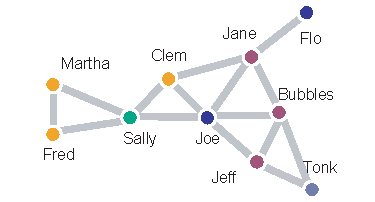
\includegraphics{images/GSpaceExampleGraph}
  \caption{Example email network.}
  \label{fig:GSpaceExampleGraph}
\end{figure}

To demonstrate the LDE, we will use the simple graph shown in
Figure~\ref{fig:GSpaceExampleGraph}.  Assume that the user wishes to
display the meta-relationship between vertices ``Martha'' and ``Tonk.''

\begin{figure}
  \centering
  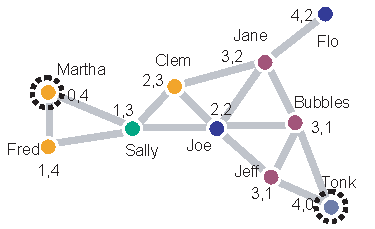
\includegraphics{images/GSpaceExampleBFS}
  \caption[Using shortest path lengths for coordinates.]{Giving coordinates
    to the graph vertices based on their shortest path distance from pivot
    points.}
  \label{fig:GSpaceExampleBFS}
\end{figure}

\index{BFS|see{breadth-first search}}

The LDE process selects those two vertices as pivot points and conducts a
breadth-first search\index{breadth-first~search} (BFS) from each. Each BFS
tags the vertices it visits with the length of the shortest path the the
start vertex. Every vertex now has an associated two-tuple containing its
shortest-path distance from each of the two pivot points as shown in
Figure~\ref{fig:GSpaceExampleBFS}.

\begin{figure}
  \centering
  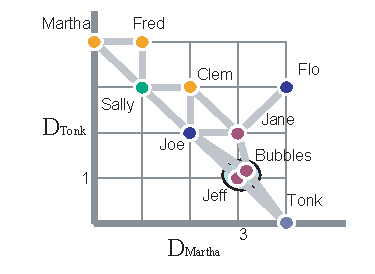
\includegraphics{images/GSpaceExamplePlot}
  \caption[Direct mapping of graph distance.]{Direct mapping of graph
    distance (length of the unweighted shortest path) as coordinates into
    two dimensional space.}
  \label{fig:GSpaceExamplePlot}
\end{figure}

Using these tuples we simply map each vertex into two dimensional geometric
space as shown in Figure~\ref{fig:GSpaceExamplePlot}.  You can see from
Figures~\ref{fig:GSpaceExampleBFS} and \ref{fig:GSpaceExamplePlot} that the
``Jeff'' and ``Bubbles'' vertices both have distance coordinates of 3,1
from the pivot points (a many-to-one mapping in the embedding
process). Where HDE resolves these many-to-one mappings using higher
dimensions and principle components analysis (PCA), LDE accepts the
many-to-one mappings and resolves them using a different technique (which
we address later). The advantage to this approach is that there is no need
to run 50 or 100 breadth-first searches (BFS), embed the graph into a 100
dimensional space, do a PCA, compute projections with maximal variance and
then project down to two dimensions.

\begin{figure}
  \centering
  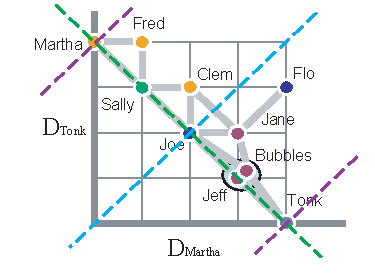
\includegraphics{images/GSpaceExampleFeatures}
  \caption{Low dimensional embedding feature lines.}
  \label{fig:GSpaceExampleFeatures}
\end{figure}

The simplicity of the low dimensional embedding exposes many interesting
geometric properties within the layout as shown in
Figure~\ref{fig:GSpaceExampleFeatures}.  The embedding based on
graph-theoretical distance ensures that the shortest path between the pivot
points is guaranteed to be along the dashed green line. Longer paths form
``arcs'' into the positive quadrant.  The light blue line represents
shortest path equidistance between the pivot points. ``Flo'' has a shorter
path to ``Tonk'' than to ``Martha'' simply based on this geometric
property.  The distance from a vertex to a pivot vertex can never be
greater than its distance to the other pivot vertex plus the shortest path
between the pivots. Thus, the two darker purple lines mark the
``boundaries'' of the layout.

\begin{figure}
  \centering
  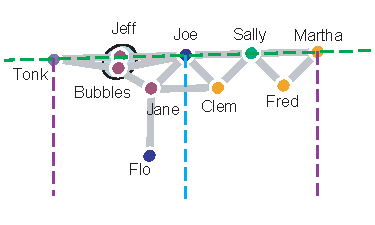
\includegraphics{images/GSpaceExampleRotated}
  \caption{LDE plot rotated 135 degrees.}
  \label{fig:GSpaceExampleRotated}
\end{figure}

Rotating the graph 135 degrees, as demonstrated in
Figure~\ref{fig:GSpaceExampleRotated}, provides a more natural
orientation.  The shortest path will be along the top and equidistance is
the vertical line in the center.

\index{Low~Dimensional~Embedding|)}

\subsubsection{Generalizing the LDE Process}

The previous example uses a point-to-point query where the two pivot points
for the LDE were specified by the user. As mentioned in the HDE work, pivot
points can be automatically computed. In our case, we run a total of three
BFS searches. The first BFS begins at a random vertex within the graph,
finds a \keyterm{pseudo-peripheral vertex}\index{pseudo-peripheral~vertex},
a vertex that has a long shortest path but is not guaranteed to be the
longest.  The pseudo-peripheral vertex is chosen simply as one of the
vertices furthest from the initial random pick.  The pseudo-peripheral
vertex becomes one of the pivot points and is passed as the starting-point
for the second BFS.  The second BFS provides vertices with the first
component of their graph distance tuple, and identifies a second
pseudo-peripheral vertex to use as the second pivot point.. This vertex
becomes the starting-point for the third BFS, which provides each vertex
with the second component of the distance tuple. The running time of this
phase is $O(|V|+|E|)$ where $|V|$ and $|E|$ are the number of vertices and
edges in the graph, respectively.

\begin{figure}
  \centering
  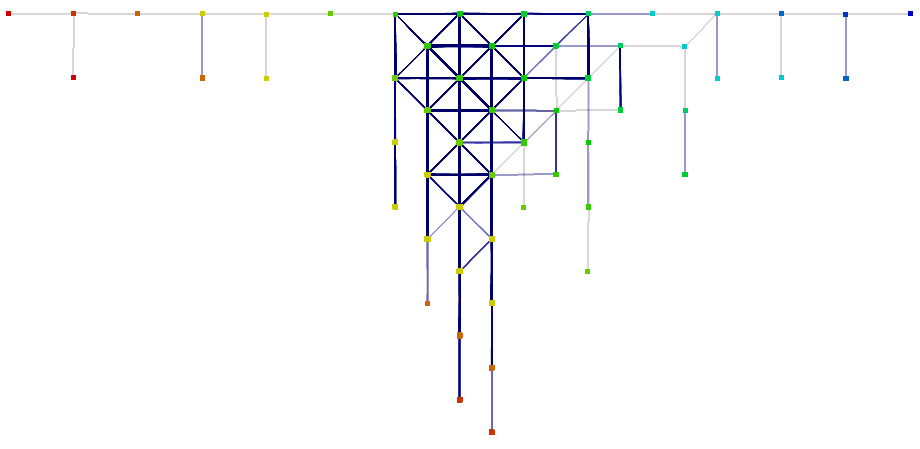
\includegraphics[width=4in]{images/GSpaceEnron}
  \caption[Automatic LDE layout of the Enron email database.]{Automatic LDE
    layout of the Enron email database (322k edges, 75k
    vertices)\lcite{Klimt04}.}
  \label{fig:GSpaceEnron}
\end{figure}

In our testing the algorithm appeared fairly insensitive to the particular
choice of peripheral vertices; initially we had been more formal about the
pivot choices. In fact, the normal procedure for finding pseudo-peripheral
vertices is to conduct a series of BFS passes until the passes give
convergence on the two pivot points. Figure~\ref{fig:GSpaceEnron}
demonstrates the layout resulting from the generalized LDE process with
automatic pivot calculation.

\subsubsection{Resolving the Many-to-One Mappings}

\index{vertex~bundling|(}

Inspired by the terrific edge bundling technique of Holten\scite{Holten06},
we adopted the term \keyterm{vertex bundling} to describe how vertices can
be packed together based on their connectivity attributes. Vertices have
edge obligations to other vertices; if you have the same obligations as
another set of vertices, bundle yourself together and \emph{minimize} the
space you take up.

\begin{figure}
  \centering
  \subfigure[Typical Force Directed Space Filling]{
    \label{fig:GSpaceVertexBundles:ForceDirected}
    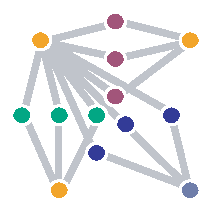
\includegraphics{images/GSpaceVBForceDirected}
  }
  \qquad
  \subfigure[Space Minimizing Vertex Bundles]{
    \label{fig:GSpaceVertexBundles:VertexBundles}
    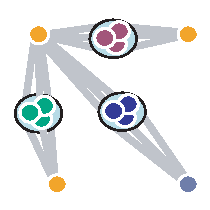
\includegraphics{images/GSpaceVBVertexBundles}
  }
  \caption[Simplifying graph layout with vertex bundles.]{Simplifying graph
    layout, and clarifying topological relationships with the use of vertex
    bundles.}
  \label{fig:GSpaceVertexBundles}
\end{figure}

If you take the small graph in Figure~\ref{fig:GSpaceVertexBundles}, you
see that traditionally the vertices are pushed apart to fill the available
space. We suggest the opposite approach, grouping the vertices together
into ``semantic'' bundles which, like the edge bundling technique, simplify
the layout and bring clarity to the topological relationships within the
graph.

On the large scale, vertex bundling can be used to resolve a significant
portion of our many-to-one mapping problem. We now use the problematic
distance bins as an ally to create a ``scaffolding'' of control
points. Each vertex has an edge to one of more other vertices, at this
point all vertices lie within a bin (control point), so we simply traverse
the vertex list, determining which vertices have edges to which control
points and bundle all vertices with edges to the same control points.

\begin{figure}
  \centering
  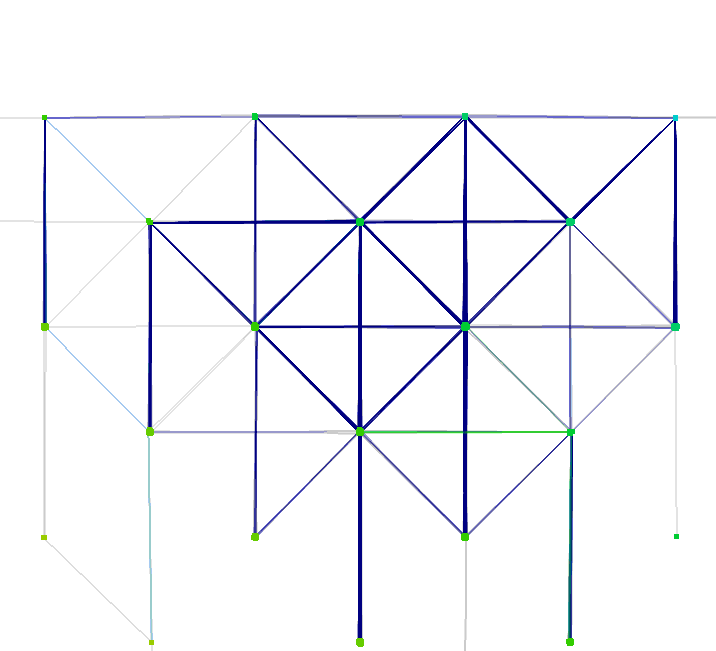
\includegraphics[width=2in]{images/GSpaceBundlingOriginal}
  \qquad
  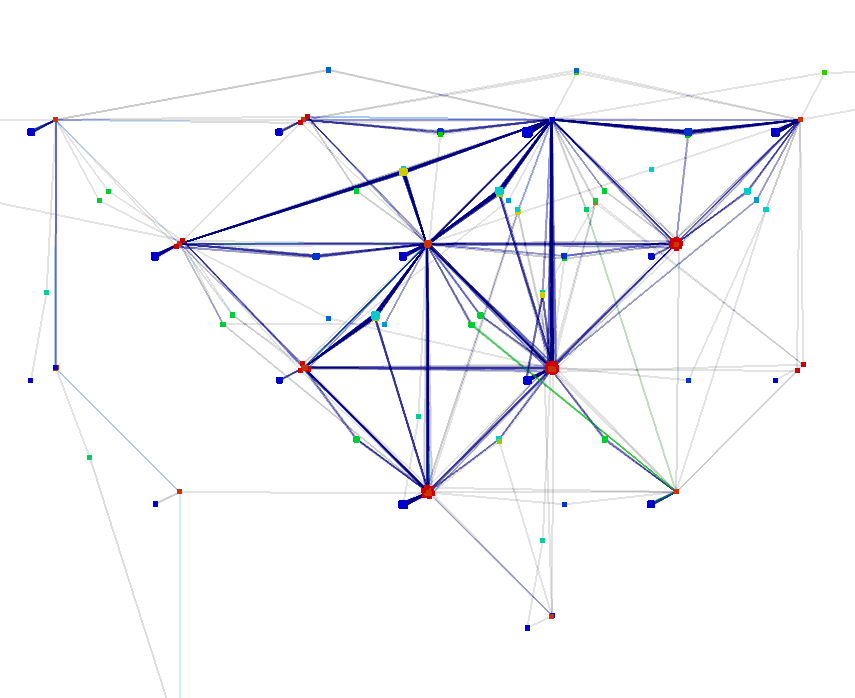
\includegraphics[width=2in]{images/GSpaceBundlingBreakout}
  \caption[Applying vertex bundling.]{ On the left an LDE layout of a
    subset of the Enron database (1374 Vertices, 2241 Edges). On the right
    the same layout after the vertex bundling pass. Vertex bundling
    significantly mitigates the many-to-one mappings and helps convey
    topological information.}
  \label{fig:GSpaceBundling}
\end{figure}

After the graph has been through the LDE phase and looks like the layout
shown on the left side of Figure~\ref{fig:GSpaceBundling}, we now pass the
graph through the vertex bundling process and in a manner similar to
marching cubes, each vertex has its edges tested against a case table of
control points to see which vertex bundle it will be a member of. The
entire graph is processed from first vertex to last, and depending on which
case is matched the vertex is offset some relative amount from its
current position. The running time of this phase is $O(|V|+|E|)$.

\begin{figure}
  \centering
  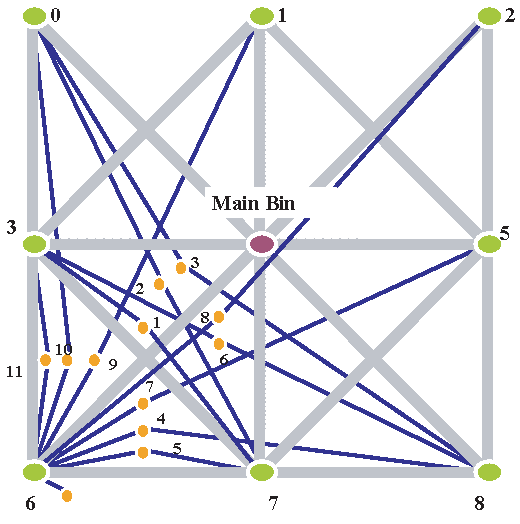
\includegraphics{images/GSpaceBundleMap}
  \caption[Vertex bundle Map.]{Vertex bundle Map. For each distance bin
    created by the LDE, the following vertex bundle map is applied.}
  \label{fig:GSpaceBundleMap}
\end{figure}

Currently we call out 14 different cases (and 11 additional sub-cases) that
are split out from the LDE bins as shown in
Figure~\ref{fig:GSpaceBundleMap}. The 25 defined cases are as follows. For
each vertex the following are determined:

\begin{enumerate}
\item Edges only go to vertices in 1 bin: case 0.
\item Edges go to vertices of 2 bins: cases 1 - 11.
\item If you are case 1-11 and also have edges back to the main bin then
  you are placed very close to your bundle but biased toward the main bin
  (see inset of Figure~\ref{fig:GSpaceBundlingInsets}): cases 12 - 22.
\item If you do not meet any of these 23 cases, but you have one or more
  edge connections within the same bin you stay in the bin: case 23.
\item If none of these apply then you are marked as an ``unresolved
  vertex'' and placed in the main bin.
\end{enumerate}

\begin{figure}
  \centering
  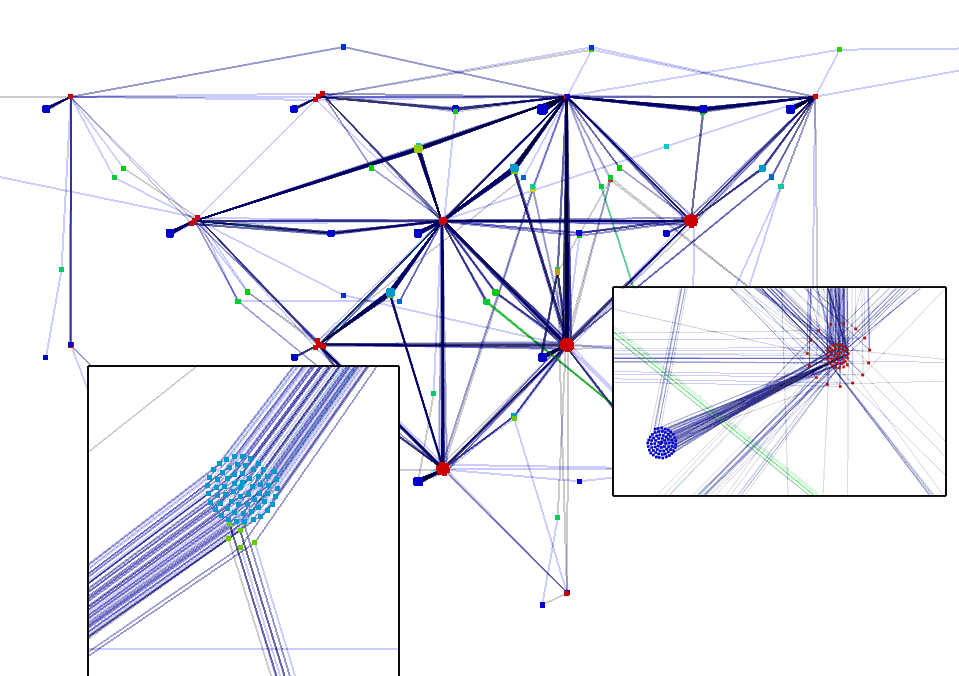
\includegraphics[width=4in]{images/GSpaceBundlingInsets}
  \caption[Vertex bundling breakout with layout detail.]{Enlarged image of
    vertex bundling breakout (left side of Figure~\ref{fig:GSpaceBundling}
    with insets showing layout detail.}
  \label{fig:GSpaceBundlingInsets}
\end{figure}

The diagram in Figure~\ref{fig:GSpaceBundleMap}, at first looks oddly
biased towards the bottom left corner. When splitting out the vertex
bundles an even distribution seems more effective, until the realization
that these bundle maps are applied at every bin within the LDE layout. So
the diagram will need to mesh well when placed next to, above, and below
your neighbors who are also applying the diagram to their vertices.

\index{vertex~bundling|)}

\subsubsection{Parallelizing the G-Space Layout}

We have not yet had a chance to implement it, but performing a G-Space
layout in parallel is straightforward and efficient.  All the major pieces
for doing this are given by Yoo et al.\scite{Yoo05} and are already
implemented in \titan.

The majority of the layout algorithm involves performing breadth-first
searches\index{breadth-first~search}.  Yoo's algorithm is proven to be
scalable and efficient on distributed memory machines.  The vertex bundling
and breakout requires only knowing the bin of the nearest neighbors.  This
information can be achieved with a limited amount of communication with the
edge partitioning\index{edge~partitioning} described in
Chapter~\ref{sec:ParallelGraphVisualizationFramework:DataStructures}.

\subsubsection{Results}

\begin{figure}
  \centering
  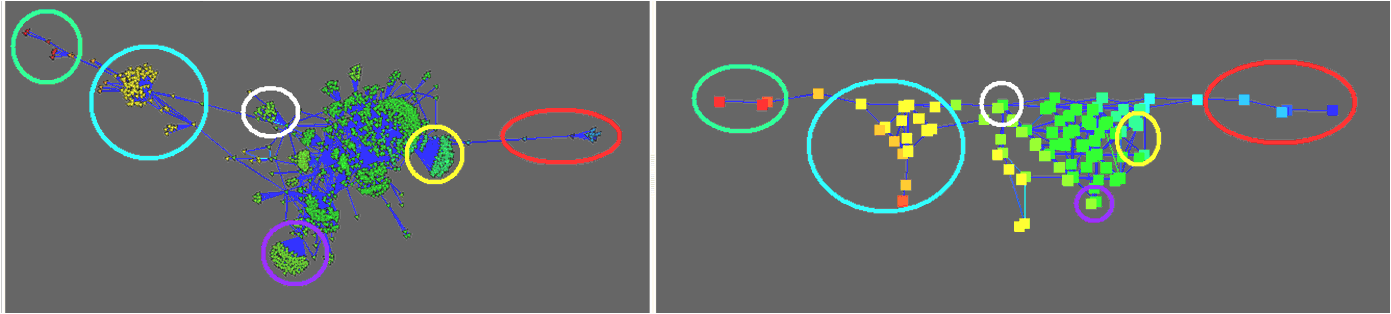
\includegraphics[width=5in]{images/GSpaceComparison}
  \caption[Correlation of the G-Space layout to force directed
    layout.]{Correlation of the G-Space layout to a traditional force
    directed layout.  Color matched circles represent similar sets of
    vertices between the two layouts. Data: subset of Enron database (1374
    Vertices, 2241 Edges).}
  \label{fig:GSpaceComparison}
\end{figure}

The quality of the visual layout of G-Space is hard to quantify when
comparing it to other layout techniques. The angular lines and extremely
tight clusters give the appearance that the layout is showing a small
graph, and so we wanted to give some visual registration with
Figure~\ref{fig:GSpaceComparison}. The color matched circles enclose the
same vertex sets in both layouts. The dataset shown is a subset of the
Enron email database (1374 Vertices, 2241 Edges). The remarkable
correlation between the visual appearances of the layouts is partially
because they were rotated and scaled to better show cluster similarity.

On a qualitative level, when exploring the two layouts side by side, with
linked selection, the G-Space layout conveys better global graph structure
and allows more detailed inspection of topological relationship.

\index{G-Space|)}

\index{graph~layout|)}

\section{Edge Accumulation}
\label{sec:EdgeAccumulation}

\section{Landscape View}
\label{sec:LandscapeView}

\section{Peak Identification and Labeling}
\label{sec:PeakIdentificationAndLabeling}


\chapter{Future Work}
\label{chap:FutureWork}


%% \chapter{Junk}

%% \begin{table}[ht]
%%   \centering
%%   \caption[Short Title]{Full caption}
%%   \bigskip

%%   \begin{tabular}{|l|c|l|c|}
%%   \end{tabular}
%%   \label{tab:1}
%% \end{table}

%% \begin{figure}[ht]
%%   \centering
%%   \subfigure[Short title]{
%%     \label{fig:sub:1}
%% %    \includegraphics[keepaspectratio=true, width= in]{filename}
%%   }
%%   \subfigure[Short title]{
%%     \label{fig:sub:2}
%% %    \includegraphics[keepaspectratio=true, width= in]{filename}
%%   }
%%   \caption{Full caption.}
%%   \label{fig:1}
%% \end{figure}



% ---------------------------------------------------------------------- %
% References
% 
\cleardoublepage
% If hyperref is included, then \phantomsection is already defined.
% If not, we need to define it.
\providecommand*{\phantomsection}{}
\phantomsection
\addcontentsline{toc}{chapter}{References}
\bibliographystyle{plain}
\bibliography{LDRD2006}


%% % ---------------------------------------------------------------------- %
%% % 
%% \appendix
%% \chapter{}

\clearpage
\addcontentsline{toc}{chapter}{\indexname}
\printindex

\begin{SANDdistribution}[NM]% or [CA]
  % \SANDdistCRADA	% If this report is about CRADA work
  % \SANDdistPatent	% If this report has a Patent Caution or Patent Interest
  % \SANDdistLDRD	% If this report is about LDRD work

  % External Address Format: {num copies}{Address}
  \SANDdistExternal{}{}
  \bigskip

  % The following MUST BE between the external and internal distributions!
  % \SANDdistClassified % If this report is classified

  % Internal Address Format: {num copies}{Mail stop}{Name}{Org}
  \SANDdistInternal{}{}{}{}

  % Mail Channel Address Format: {num copies}{Mail Channel}{Name}{Org}
  \SANDdistInternalM{}{}{}{}
\end{SANDdistribution}


% The second printing
% \begin{SANDreDistribution}
%   \SANDdistExternal{}{}
%   \bigskip
%   \SANDdistInternal{}{}{}{}
%   \SANDdistInternalM{}{}{}{}
% \end{SANDreDistribution}

\end{document}
